   %% LyX 2.3.4.2 created this file.  For more info, see http://www.lyx.org/.
%% Do not edit unless you really know what you are doing.
\documentclass[12pt,oneside,american,czech]{book}
\usepackage[T1]{fontenc}
\usepackage[utf8]{inputenc}
\usepackage[a4paper]{geometry}
\geometry{verbose,tmargin=4cm,bmargin=3cm,lmargin=3cm,rmargin=2cm,headheight=0.8cm,headsep=1cm,footskip=0.5cm}
\pagestyle{headings}
\setcounter{secnumdepth}{3}
\usepackage{url}
\usepackage{amsmath}
\usepackage{amsthm}
\usepackage{amssymb}
\usepackage{graphicx}
\usepackage{setspace}
\usepackage{hyperref}
\usepackage{libertine}
\usepackage{comment}
\usepackage{calrsfs}
\usepackage{subfig}
\usepackage{cite}
\usepackage{url}
\usepackage[linesnumbered,ruled,vlined]{algorithm2e}
\usepackage{algpseudocode}
\usepackage{tikz}
\makeatletter
%%%%%%%%%%%%%%%%%%%%%%%%%%%%%% Textclass specific LaTeX commands.
\newenvironment{lyxlist}[1]
	{\begin{list}{}
		{\settowidth{\labelwidth}{#1}
		 \setlength{\leftmargin}{\labelwidth}
		 \addtolength{\leftmargin}{\labelsep}
		 \renewcommand{\makelabel}[1]{##1\hfil}}}
	{\end{list}}

%%%%%%%%%%%%%%%%%%%%%%%%%%%%%% User specified LaTeX commands.
%% Font setup: please leave the LyX font settings all set to 'default'
%% if you want to use any of these packages:

%% Use Times New Roman font for text and Belleek font for math
%% Please make sure that the 'esint' package is turned off in the
%% 'Math options' page.
\usepackage[varg]{txfonts}

%% Use Utopia text with Fourier-GUTenberg math
%\usepackage{fourier}

%% Bitstream Charter text with Math Design math
%\usepackage[charter]{mathdesign}

%%---------------------------------------------------------------------

%% Make the multiline figure/table captions indent so that the second
%% line "hangs" right below the first one.
%\usepackage[format=hang]{caption}

%% Indent even the first paragraph in each section
\usepackage{indentfirst}

%%---------------------------------------------------------------------

%% Disable page numbers in the TOC. LOF, LOT (TOC automatically
%% adds \thispagestyle{chapter} if not overriden
%\addtocontents{toc}{\protect\thispagestyle{empty}}
%\addtocontents{lof}{\protect\thispagestyle{empty}}
%\addtocontents{lot}{\protect\thispagestyle{empty}}

%% Shifts the top line of the TOC (not the title) 1cm upwards 
%% so that the whole TOC fits on 1 page. Additional page size
%% adjustment is performed at the point where the TOC
%% is inserted.
%\addtocontents{toc}{\protect\vspace{-1cm}}

%%---------------------------------------------------------------------

% completely avoid orphans (first lines of a new paragraph on the bottom of a page)
\clubpenalty=9500

% completely avoid widows (last lines of paragraph on a new page)
\widowpenalty=9500

% disable hyphenation of acronyms
\hyphenation{CDFA HARDI HiPPIES IKEM InterTrack MEGIDDO MIMD MPFA DICOM ASCLEPIOS MedInria}

%%---------------------------------------------------------------------

%% Print out all vectors in bold type instead of printing an arrow above them
\renewcommand{\vec}[1]{\boldsymbol{#1}}
\newcommand{\R}{\mathbb{R}}
\newtheorem{theorem}{Theorem}
\newtheorem*{poz}{Poznámka}
\theoremstyle{definition}
\newtheorem{definition}{Definition}
\newtheorem{vet}{Věta}[section]
\newtheorem*{pří}{Příklad}
\newcommand{\N}{\mathbb{N}}
\newcommand{\C}{\mathbb{C}}
\newcommand{\Z}{\mathbb{Z}}
%  Matematika
\newcommand{\ee}{\mathrm{e}} %eulerovo číslo
\newcommand{\ii}{\mathrm{i}} %imaginární jednotka
\newcommand{\E}{\mathbb{E}} %eulerovo číslo
\newcommand{\inR}{\in \mathbb{R}}
\newcommand{\dd}{\mathrm{d}}
\newcommand\KLDeq{\mathrel{\stackrel{\makebox[0pt]{\mbox{\normalfont\tiny KLD}}}{\approx}}}
\newcommand*{\matr}[1]{\mathbfit{#1}}
\newcommand*{\tran}{^{\mkern-1.5mu\mathsf{T}}}
\newcommand*{\conj}[1]{\overline{#1}}
\newcommand*{\hermconj}{^{\mathsf{H}}}
\DeclareMathOperator{\tr}{tr}
\DeclareMathOperator*{\argmin}{arg\,min} 
\DeclareMathOperator*{\argmax}{arg\,max} 
\DeclareMathAlphabet{\pazocal}{OMS}{zplm}{m}{n}
% Jednotky
\newcommand{\unit}[1]{\,\mathrm{#1}} %jednotky zadávejte pomocí tohoto příkazu
\renewcommand{\deg}{\ensuremath{\mathring{\;}}} %symbol stupně
\newcommand{\celsius}{\ensuremath{\deg\mathrm{C}}} %stupně celsia

%(hodnota plus mínus chyba) jednotka
\newcommand{\hodn}[3]{(#1 \pm #2)\unit{#3}} 
\newcommand\norm[1]{\left\lVert#1\right\rVert}
%veličina [jednotka] do hlavičky tabulky
\newcommand{\tabh}[2]{\ensuremath{#1\,[\mathrm{#2}]}} 
% Replace standard \cite by the parenthetical variant \citep
%\renewcommand{\cite}{\citep}
\newcommand{\diag}{\mathop{\mathrm{diag}}}
\def\Var{{\textrm{Var}}\,}



\makeatother

\usepackage{babel}
\begin{document}
\section*{Cross-Validation}
Probably the simplest and most widely used method for estimating prediction error is \textit{cross-validation}. This method directly estimates the expected extra-sample error 
\begin{equation}
\mathrm{Err} = \E\left[L\left(Y, \hat{f}\left(X\right)\right)\right],
\end{equation}
the average generalization error when the method $\hat{f}\left(X\right)$ is applied to an independent test sample form the joint distribution of $X$ and $Y$- As mentioned earlier, we might hope that cross-validation estimates the conditional error, with the training set $\pazocal{T}$ held fixed. But cross-validation typically estimates well only the expected prediction error.

\subsection*{K-Fold Cross-Validation}
Ideally, if we had enough data, we would set aside a validation set and use
it to assess the performance of our prediction model. Since data are often
scarce, this is usually not possible. To finesse the problem, K-fold cross-validation
uses part of the available data to fit the model, and a different
part to test it. We split the data into $K$ roughly equal-sized parts; for
example, when $K = 5$, the scenario looks like this: \\

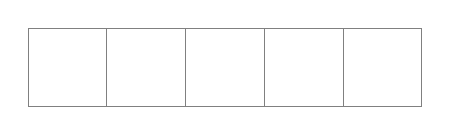
\begin{tikzpicture}
\draw[step=1cm,gray,very thin] (0,0) grid (5,1);
\end{tikzpicture}

For the $k$th part (third above), we fit the model to the other $K-1$ parts
of the data, and calculate the prediction error of the fitted model when
predicting the $k$th part of the data. We do this for $k = 1,2,\dots,K$ and
combine the $K$ estimates of prediction error.\\
Here are more details. Let $\kappa : \left\lbrace 1,\dots,N\right\rbrace\rightarrow  \left\lbrace 1,\dots,K\right\rbrace$ be an indexing
function that indicates the partition to which observation $i$ is allocated by
the randomization. Denote by $\hat{f}^{-k}\left(x\right)$ the fitted function, computed with
the $k$th part of the data removed. Then the cross-validation estimate of
prediction error is
\begin{equation}
\mathrm{CV}\left(\hat{f}\right) = \frac{1}{N}\sum_{i = 1}^{N}L\left(y_i , \hat{f}^{-\kappa\left(i\right)}\left(x_i\right)\right).
\end{equation}

\end{document}